\documentclass[11pt,a4paper]{article}

\usepackage[T1]{fontenc}
\usepackage{lmodern}
\usepackage[margin=2cm]{geometry}
\usepackage{microtype}
\usepackage{amsmath}
\usepackage{booktabs}
\usepackage{graphicx}
\usepackage{caption}
\usepackage{enumitem}
\usepackage{fancyvrb}
\usepackage{xcolor}
\usepackage{placeins}
\usepackage[colorlinks,allcolors=blue!50!black]{hyperref}

\captionsetup{font=small,labelfont=bf,skip=4pt}
\setlist{itemsep=1pt,topsep=3pt}
\setlength{\parskip}{3pt}
\setlength{\parindent}{0pt}

% Generated by cae.report_assets - do not edit by hand.
\newcommand{\NWeeks}{577}
\newcommand{\NEtfs}{25}
\newcommand{\NCandidates}{40}
\newcommand{\NDeveloped}{12}
\newcommand{\NEmerging}{13}
\newcommand{\LSWeekly}{$-$0.073}
\newcommand{\LSAnn}{$-$3.8}
\newcommand{\LSt}{$-$1.51}
\newcommand{\LSSharpe}{$-$0.45}
\newcommand{\NetAnn}{$-$17.3}
\newcommand{\Nett}{$-$6.88}
\newcommand{\TurnoverPerSide}{85}
\newcommand{\CostAnn}{13.5}
\newcommand{\HighAnn}{7.4}
\newcommand{\MiddleAnn}{9.6}
\newcommand{\LowAnn}{11.2}
\newcommand{\FMasv}{$-$0.030}
\newcommand{\FMasvt}{$-$1.49}
\newcommand{\FMasvc}{$-$0.011}
\newcommand{\FMasvct}{$-$0.54}
\newcommand{\AlphaAnn}{$-$4.0}
\newcommand{\Alphat}{$-$1.56}
\newcommand{\AlphaRsq}{0.8}
\newcommand{\PlaceboP}{0.09}
\newcommand{\PlaceboPct}{9}
\newcommand{\RoneFourt}{$-$2.01}
\newcommand{\PremMKT}{0.139}
\newcommand{\PremMOM}{$-$0.008}
\newcommand{\PremREV}{0.120}
\newcommand{\PremUSD}{0.059}
\newcommand{\PremMKTt}{1.40}
\newcommand{\PremMOMt}{$-$0.13}
\newcommand{\PremREVt}{2.02}
\newcommand{\PremUSDt}{1.63}
\newcommand{\LOOtMin}{$-$1.90}
\newcommand{\LOOtMax}{$-$1.17}
\newcommand{\RobNegative}{11}
\newcommand{\RobTotal}{13}

\newcommand{\repourl}{https://github.com/Corentin00/country-attention-etfs}
\newcommand{\todo}[1]{\textcolor{red}{[#1]}}
\newcommand{\refto}[2]{\hyperlink{ref:#1}{#2}}

\title{\vspace{-1.5cm}\textbf{Does the World's Attention Move Country Markets?}\\[2pt]
\large Wikipedia page views and the cross-section of country ETF returns}
\author{Corentin Caillaud \\ \small Hedge Fund Club St.\ Gallen --- Systematic track}
\date{\small October 2026 \quad$\cdot$\quad Code, data and frozen specification: \url{\repourl}}

\begin{document}
\maketitle
\vspace{-0.6cm}

\noindent\textbf{Summary.}
I test whether abnormal English Wikipedia attention to a country predicts the relative weekly
returns of its iShares MSCI ETF, using \NEtfs{} liquid country ETFs over \NWeeks{} weeks
(2015--2026) and a specification frozen before any return was computed. High-attention
countries underperform low-attention ones by \LSLoss\% per year, but the spread is not
significant (Newey--West $t=\LSt$), vanishes once past returns are controlled for, is not
explained by known factors, and is matched by \PlaceboPct\% of random placebo signals.
Because attention is short-lived, about \TurnoverPerSide\% of each side is replaced every week
and the strategy loses \NetLoss\% per year after costs. I would not trade it.

% =====================================================================================
\section{Economic thesis}
Do bursts of public attention to a country move the price of its equity ETF? I test three
hypotheses, which differ in the sign and the timing of the effect.

\textbf{H0: attention is already in prices.} Page views are public, so professional investors can
watch them as easily as I can; if attention predicted returns, they would already trade on it and
arbitrage the effect away. Abnormal attention then does not predict returns.

\textbf{H1: price pressure.} When a country's page draws unusual attention, inexperienced investors
are reading about it to inform themselves before buying its ETF. Their buying pushes the ETF slightly
above fair value, so high-attention countries outperform for a week or two and then give the gain
back \refto{barber2008}{(Barber \& Odean, 2008}; \refto{da2011}{Da, Engelberg \& Gao, 2011)}.

\textbf{H2: risk premium.} Attention spikes often signal a crisis. When a country suddenly looks
riskier, investors sell until the price is low enough that the expected future return pays them for
holding the risk, so high-attention countries earn \emph{higher} returns afterwards, and the gain
persists.

H0 excludes H1 and H2, but H1 and H2 do not strictly rule each other out: both can be partly true.
The horizon profile of the High-minus-Low spread shows which one dominates: a full reversal points
to H1, no reversal to H2, and a partial reversal to a mix. Existing evidence concerns individual
stocks and Google searches; here the question is asked for whole countries, using Wikipedia page
views and tradable ETFs.

% =====================================================================================
\section{Data and signal construction}

\textbf{Data.} Daily English Wikipedia page views come from the Wikimedia REST API
(\texttt{agent=user}, which excludes identified bots), available from 1 July 2015.
ETF prices are daily adjusted closes from Yahoo Finance, so returns include dividends.
The risk-free rate is from the Ken French Data Library; the US dollar is proxied by the UUP ETF.
All data is free and the raw downloads are committed to the repository.

\textbf{Universe.} I start from all \NCandidates{} iShares MSCI single-country ETFs (US
included) and keep those launched before 1 July 2015 whose median daily dollar volume was at
least \$5M over July 2014--June 2015. Measuring liquidity \emph{before} the sample avoids
selecting ETFs that later became popular. The \$5M threshold is a judgment call: at that
volume a position of a few hundred thousand dollars is below 5\% of one day's trading, and bid--ask
spreads stay within the cost assumption of Section~\ref{sec:perf}; the principle of excluding
illiquid assets follows \refto{novymarx2016}{Novy-Marx \& Velikov (2016)} and
\refto{hou2020}{Hou, Xue \& Zhang (2020)}. \NEtfs{} ETFs pass (\NDeveloped{} developed,
\NEmerging{} emerging markets). The US ETF (EUSA) fails the liquidity rule, and Russia (ERUS)
is missing because its price history was deleted after the 2022 suspension
(Appendix~\ref{app:universe}).

\textbf{Signal.} Weeks run Monday to Sunday (UTC), the time zone in which Wikimedia counts daily
views, so the Sunday cut-off is unambiguous. For country $i$ and week $w$, let $V_{i,w}$
be the sum of the seven daily views of the country's Wikipedia page. Abnormal attention, ASV (``abnormal search volume'', the name
\refto{da2011}{Da, Engelberg \& Gao (2011)} give to the same measure built from Google searches), is
\begin{equation*}
  \mathrm{ASV}_{i,w} \;=\; \ln\left(V_{i,w}\right) \;-\; \ln\left(\operatorname{median}\left(V_{i,w-1},\dots,V_{i,w-8}\right)\right).
\end{equation*}
The log difference makes large and small countries comparable (India's page has six times the
traffic of Chile's), and the median of the previous eight weeks, taken from \refto{da2011}{Da, Engelberg \& Gao
(2011)}, adapts to slow trends such as the secular decline of Wikipedia traffic while ignoring
one-off spikes. Portfolios use only the cross-sectional rank of ASV, so extreme weeks cannot
dominate. Figure~\ref{fig:signal} in the appendix shows the signal around the Brexit vote.

\textbf{Timing and sample.} The signal uses views up to Sunday 24:00 UTC; positions are opened
at the close of the next US trading day and held one week, so there is no look-ahead. The sample
runs from the signal week ending 6 September 2015 (the first with eight weeks of history) to the
week ending 20 September 2026: \NWeeks{} weeks. The full specification, including the robustness
list and the decision rule, was frozen and time-stamped on 3 October 2026 before any return was
computed (Appendix~\ref{app:spec}).

% =====================================================================================
\section{Strategy}
\begin{enumerate}[leftmargin=*]
  \item Universe: the \NEtfs{} ETFs of Appendix~\ref{app:universe}.
  \item Every Monday before the US close, download the previous week's (Monday--Sunday UTC) daily
        English Wikipedia views (\texttt{agent=user}) of each country page, plus the eight weeks before it.
  \item For each country compute $V$ = last week's total views, $B$ = median of the eight previous
        weekly totals, and $\mathrm{ASV} = \ln(V) - \ln(B)$.
  \item Rank the $N$ countries by ASV. The $\lfloor N/3\rfloor$ countries with the highest ASV form
        \emph{High} and the $\lfloor N/3\rfloor$ with the lowest form \emph{Low} (8 each with
        25 countries); the remaining countries are not traded.
  \item At the Monday close (Tuesday if Monday is a US holiday), buy every High ETF and short every
        Low ETF, with equal dollar amounts per ETF and equal total dollars on each side.
  \item Hold one week; at the next rebalance close repeat steps 2--5 and trade only the differences.
  \item If an ETF is suspended or delisted, its position can no longer be traded: value it at
        its last traded price, remove the ETF from future rankings, and book the liquidation
        proceeds when the issuer pays them.
\end{enumerate}

% =====================================================================================
\section{Performance evaluation}\label{sec:perf}

Table~\ref{tab:main} reports the three tercile portfolios and the long--short spread.
The ordering is monotonic but in the \emph{opposite} direction to H1 and H2: High earns
\HighAnn\% per year, Middle \MiddleAnn\% and Low \LowAnn\%. The spread of \LSAnn\% per year is not
significant ($t=\LSt$, Sharpe \LSSharpe). The horizon profile (Figure~\ref{fig:main}b) shows
neither the rise-and-reversal predicted by price pressure (H1) nor a persistent positive spread
(H2): no single week after formation is significant and the cumulative spread drifts slowly
downward. Figure~\ref{fig:main}a shows that most of the gross loss occurs between late 2021 and 2023.

\begin{table}[h]
\centering\small
\caption{One-week holding, weekly rebalancing, September 2015--September 2026. Newey--West
$t$-statistics with four lags. Net returns deduct 10\,bp (developed) or 20\,bp (emerging) per
one-way trade.}
\label{tab:main}
\begin{tabular}{lrrrrrrr}
\toprule
 & Mean/wk & Ann. & NW $t$ & Vol & Sharpe & Max DD & Hit \\
 & \% & \% & & \% & & \% & \% \\
\midrule
High & 0.143 & 7.4 & 1.39 & 18.6 & 0.40 & $-$44 & 54 \\
Middle & 0.185 & 9.6 & 1.83 & 18.2 & 0.53 & $-$42 & 57 \\
Low & 0.216 & 11.2 & 2.09 & 18.0 & 0.62 & $-$40 & 57 \\
\midrule
High $-$ Low (gross) & $-$0.073 & $-$3.8 & $-$1.51 & 8.4 & $-$0.45 & $-$46 & 47 \\
High $-$ Low (net) & $-$0.333 & $-$17.3 & $-$6.88 & 8.4 & $-$2.06 & $-$86 & 38 \\
\bottomrule
\end{tabular}
\end{table}

\begin{figure}[h]
\centering
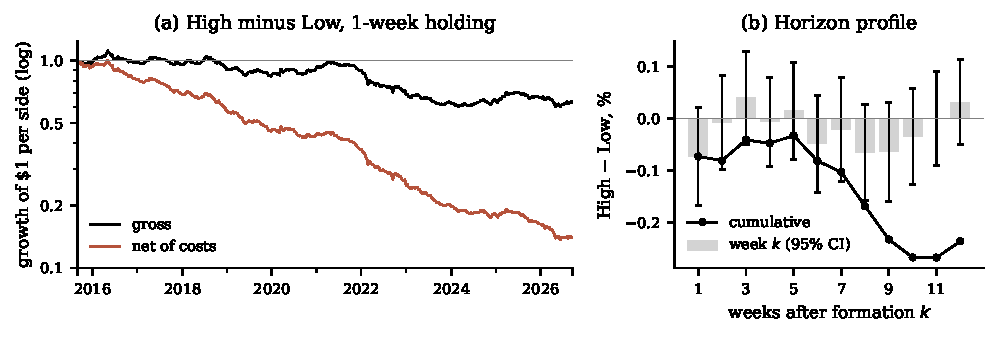
\includegraphics[width=\textwidth]{figures/fig_main.pdf}
\caption{(a) Cumulative High-minus-Low return, gross and net of costs. (b) Mean High-minus-Low
return earned in week $k$ after formation, with 95\% confidence intervals, and its cumulative sum.}
\label{fig:main}
\end{figure}

\textbf{Is attention new information?} Table~\ref{tab:newinfo} asks whether the weak negative
spread is a disguised version of known effects. In Fama--MacBeth regressions the ASV coefficient
alone is \FMasv\% per standard deviation ($t=\FMasvt$); adding past returns at three horizons,
volatility and the baseline attention level shrinks it to \FMasvc\% ($t=\FMasvct$). Attention is
slightly higher after recent losses, consistent with crises drawing readers, but this link is
weak. Against four factors built from the same universe, the alpha is \AlphaAnn\% per year
($t=\Alphat$) and the factors explain only \AlphaRsq\% of the spread's variance: it is not market,
momentum, reversal or dollar exposure, it is mostly noise. The short-term reversal factor itself
is significant in this universe (Appendix~\ref{app:tables}), which shows the setup can detect a
real cross-sectional effect.

\begin{table}[h]
\centering\small
\caption{Panel A: weekly cross-sectional regressions of next-week returns on cross-sectionally
standardized variables; time-series means with Newey--West $t$ in parentheses. Panel B:
regression of the weekly High-minus-Low return on equal-weighted universe excess return (Market),
12-1 week momentum, last-week reversal and the UUP return.}
\label{tab:newinfo}
\begin{tabular}{lrrrr}
\toprule
\multicolumn{5}{l}{\textit{Panel A: Fama--MacBeth, next-week return (\% per cross-sectional s.d.)}} \\
 & \multicolumn{2}{c}{ASV only} & \multicolumn{2}{c}{With controls} \\
\cmidrule(lr){2-3}\cmidrule(lr){4-5}
ASV rank & $-$0.030 & ($-$1.49) & $-$0.011 & ($-$0.54) \\
Return, last week &  &  & $-$0.042 & ($-$1.31) \\
Return, weeks $-4$ to $-2$ &  &  & $-$0.019 & ($-$0.62) \\
Return, weeks $-52$ to $-5$ &  &  & 0.013 & (0.39) \\
Volatility (26 weeks) &  &  & 0.017 & (0.51) \\
Baseline attention level &  &  & 0.011 & (0.62) \\
\midrule
\multicolumn{5}{l}{\textit{Panel B: High $-$ Low on four factors from the same universe}} \\
 & Coef. & ($t$) & & \\
Alpha (\% p.a.) & $-$4.01 & ($-$1.56) & & \\
Market & 0.02 & (0.67) & & \\
Momentum & $-$0.00 & ($-$0.09) & & \\
Short-term reversal & 0.04 & (0.76) & & \\
US dollar & $-$0.05 & ($-$0.51) & & \\
$R^2$ & 0.008 & & & \\
\bottomrule
\end{tabular}
\end{table}

% =====================================================================================
\section{Robustness}

All variations were fixed in the frozen specification. Figure~\ref{fig:robustness} shows that
the sign is negative in \RobNegative{} of \RobTotal{} variations but the effect is never reliable.
Only the 4-week baseline crosses $|t|=2$ ($t=\RoneFourt$), which is what one would expect by chance
among thirteen tests. The sign flips with \emph{Economy of} pages and in 2020--2021, and the spread
weakens if trades are delayed by one day. Dropping any single country leaves $t$ between \LOOtMin{}
and \LOOtMax{}, so no country drives the result, and excluding English-majority countries (whose
pages are read mostly by residents) changes little. Finally, shuffling the signal across countries
within each week 1{,}000 times produces a spread at least as extreme as the actual one in
\PlaceboP{} of cases (two-sided $p=\PlaceboP$).

\begin{figure}[h]
\centering
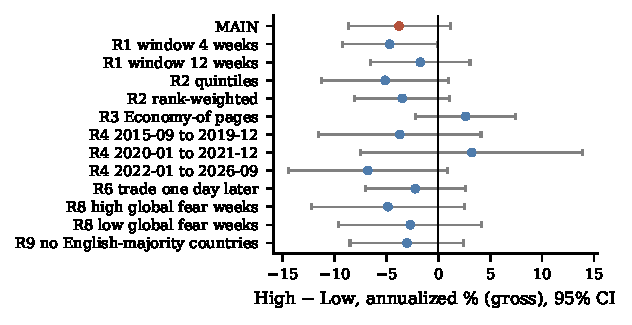
\includegraphics[width=0.62\textwidth]{figures/fig_robustness.pdf}
\caption{Annualized gross High-minus-Low return and 95\% Newey--West confidence interval for every
pre-specified variation: R1 baseline window, R2 portfolio construction, R3 \emph{Economy of}
pages, R4 sub-periods, R6 one-day trading delay, R8 global-fear regimes, R9 non-English-majority
countries. Full numbers in Table~\ref{tab:robustness}.}
\label{fig:robustness}
\end{figure}

% =====================================================================================
\section{Would I trade it?}
\todo{To be written: decision rule result (Table~\ref{tab:decision} in the appendix can be moved
here), turnover and costs as the structural obstacle, what I would try next, reflection.}

% =====================================================================================
\clearpage
\section*{References}
\small
\begin{itemize}[leftmargin=*,label={}]
  \item \hypertarget{ref:barber2008}{}Barber, B.\,M., and T.\ Odean (2008). All that glitters: the effect of
        attention and news on the buying behavior of individual and institutional investors.
        \textit{Review of Financial Studies} 21(2), 785--818. \url{https://doi.org/10.1093/rfs/hhm079}
  \item \hypertarget{ref:da2011}{}Da, Z., J.\ Engelberg, and P.\ Gao (2011). In search of attention.
        \textit{Journal of Finance} 66(5), 1461--1499. \url{https://doi.org/10.1111/j.1540-6261.2011.01679.x}
  \item \hypertarget{ref:fama1973}{}Fama, E.\,F., and J.\,D.\ MacBeth (1973). Risk, return, and equilibrium:
        empirical tests. \textit{Journal of Political Economy} 81(3), 607--636.
        \url{https://doi.org/10.1086/260061}
  \item \hypertarget{ref:hou2020}{}Hou, K., C.\ Xue, and L.\ Zhang (2020). Replicating anomalies.
        \textit{Review of Financial Studies} 33(5), 2019--2133. \url{https://doi.org/10.1093/rfs/hhy131}
  \item \hypertarget{ref:jegadeesh1993}{}Jegadeesh, N., and S.\ Titman (1993). Returns to buying winners
        and selling losers: implications for stock market efficiency. \textit{Journal of Finance}
        48(1), 65--91. \url{https://doi.org/10.1111/j.1540-6261.1993.tb04702.x}
  \item \hypertarget{ref:moat2013}{}Moat, H.\,S., C.\ Curme, A.\ Avakian, D.\,Y.\ Kenett, H.\,E.\ Stanley, and
        T.\ Preis (2013). Quantifying Wikipedia usage patterns before stock market moves.
        \textit{Scientific Reports} 3, 1801. \url{https://doi.org/10.1038/srep01801}
  \item \hypertarget{ref:newey1987}{}Newey, W.\,K., and K.\,D.\ West (1987). A simple, positive semi-definite,
        heteroskedasticity and autocorrelation consistent covariance matrix. \textit{Econometrica}
        55(3), 703--708. \url{https://doi.org/10.2307/1913610}
  \item \hypertarget{ref:novymarx2016}{}Novy-Marx, R., and M.\ Velikov (2016). A taxonomy of anomalies and
        their trading costs. \textit{Review of Financial Studies} 29(1), 104--147.
        \url{https://doi.org/10.1093/rfs/hhv063}
\end{itemize}
\normalsize

\clearpage
\appendix
\renewcommand{\thesection}{\Alph{section}}
\setcounter{figure}{0}\renewcommand{\thefigure}{A\arabic{figure}}
\setcounter{table}{0}\renewcommand{\thetable}{A\arabic{table}}

\section{Pre-registered specification}\label{app:spec}
The specification below was e-mailed to myself and committed as the first commit of the
repository (\texttt{f33a66c}, 3 October 2026, 15:17 CEST) before any return was computed.
Deviations are listed in Appendix~\ref{app:deviations}.

{\scriptsize\VerbatimInput{spec_frozen.txt}}

\section{Universe}\label{app:universe}
\begin{table}[h]
\centering\footnotesize
\caption{All candidate ETFs, sorted by median daily dollar volume over July 2014--June 2015.
DM/EM: MSCI classification as of 1 July 2015.}
\begin{tabular}{llcrl}
\toprule
ETF & Wikipedia page & Market & \$M/day & Included \\
\midrule
EWZ & Brazil & EM & 668.49 & yes \\
EWJ & Japan & DM & 331.45 & yes \\
EWY & South Korea & EM & 135.22 & yes \\
EWW & Mexico & EM & 125.45 & yes \\
EWG & Germany & DM & 123.97 & yes \\
EWT & Taiwan & EM & 103.55 & yes \\
EWH & Hong Kong & DM & 55.23 & yes \\
EWU & United Kingdom & DM & 44.48 & yes \\
EWA & Australia & DM & 41.18 & yes \\
EWC & Canada & DM & 40.49 & yes \\
EWP & Spain & DM & 40.44 & yes \\
EWI & Italy & DM & 32.64 & yes \\
INDA & India & EM & 27.70 & yes \\
EZA & South Africa & EM & 26.87 & yes \\
MCHI & China & EM & 23.09 & yes \\
EWM & Malaysia & EM & 18.37 & yes \\
THD & Thailand & EM & 16.83 & yes \\
EWL & Switzerland & DM & 15.95 & yes \\
EWQ & France & DM & 15.88 & yes \\
TUR & Turkey & EM & 15.22 & yes \\
EIDO & Indonesia & EM & 15.15 & yes \\
EWS & Singapore & DM & 11.07 & yes \\
ECH & Chile & EM & 9.16 & yes \\
EPHE & Philippines & EM & 8.11 & yes \\
EWD & Sweden & DM & 6.34 & yes \\
EPOL & Poland & EM & 4.89 & below liquidity threshold \\
EWN & Netherlands & DM & 3.61 & below liquidity threshold \\
EWK & Belgium & DM & 1.89 & below liquidity threshold \\
EPU & Peru & EM & 1.54 & below liquidity threshold \\
EIS & Israel & DM & 1.29 & below liquidity threshold \\
EIRL & Republic of Ireland & DM & 1.06 & below liquidity threshold \\
EWO & Austria & DM & 0.91 & below liquidity threshold \\
ENZL & New Zealand & DM & 0.74 & below liquidity threshold \\
EDEN & Denmark & DM & 0.63 & below liquidity threshold \\
ENOR & Norway & DM & 0.31 & below liquidity threshold \\
UAE & United Arab Emirates & EM & 0.29 & below liquidity threshold \\
EFNL & Finland & DM & 0.20 & below liquidity threshold \\
QAT & Qatar & EM & 0.13 & below liquidity threshold \\
EUSA & United States & DM & 0.12 & below liquidity threshold \\
ERUS & Russia & EM & 0.00 & no Yahoo data \\
\bottomrule
\end{tabular}
\end{table}

\begin{figure}[h]
\centering
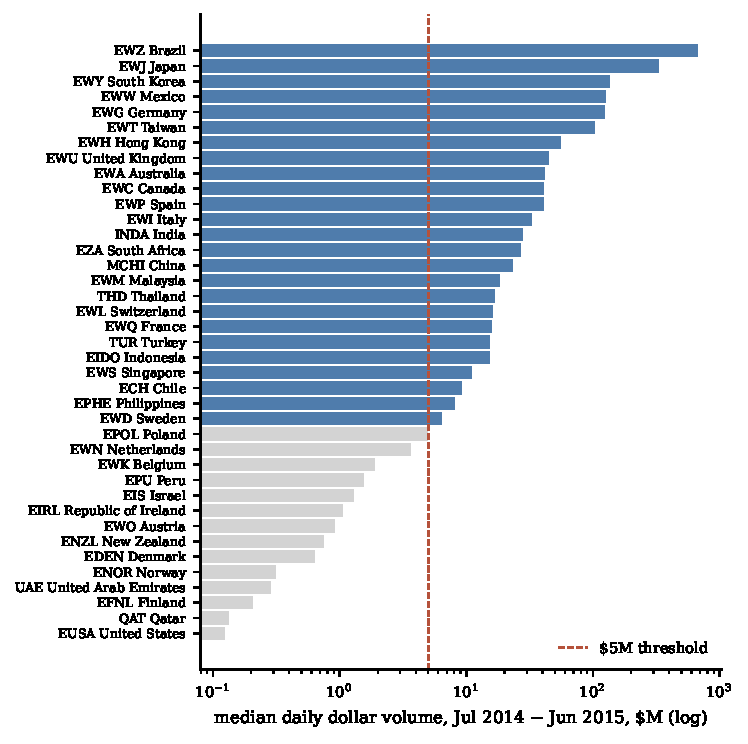
\includegraphics[width=0.75\textwidth]{figures/fig_liquidity.pdf}
\caption{Liquidity filter. Blue: included. ERUS (Russia) is not shown: Yahoo Finance no
longer has its price history, so its volume is unknown rather than zero.}
\end{figure}

\section{Deviations, implementation details and limitations}\label{app:deviations}
\textbf{Deviations from the frozen specification.}
\begin{itemize}[leftmargin=*]
  \item Decision rule (a) reads ``net-of-cost $|t|>2$''. Read literally, a significantly
        \emph{losing} strategy would pass; I apply the intended meaning, a profitable strategy as
        specified ($t>2$). The verdict is unchanged either way.
  \item Table~\ref{tab:newinfo} adds an ASV-only Fama--MacBeth column as a reference point for the
        specified regression with controls.
\end{itemize}
\textbf{Implementation details not fixed by the specification.}
\begin{itemize}[leftmargin=*]
  \item US trading days are days on which at least 90\% of the ETFs have a price.
  \item The Ken French risk-free series ends on 31 August 2026; its last value is carried forward
        for the final four weeks.
  \item Volatility is the standard deviation of daily log returns over the previous 182 calendar
        days, with at least 100 observations.
  \item The horizon profile reports both event-time returns (week $k$ after formation) and
        overlapping Jegadeesh--Titman portfolios held $h$ weeks, with Newey--West lags $\max(4,h)$.
\end{itemize}
\textbf{Limitations.}
\begin{itemize}[leftmargin=*]
  \item \emph{Survivorship:} Russia, whose ETF was suspended in 2022, is missing for lack of data.
  \item \emph{Bots:} a few spikes have no identifiable news event (e.g.\ Canada, 22 May 2017, 59 times
        the median; Singapore on 24 December of both 2016 and 2017 with near-identical counts) and are
        probably automated traffic misclassified as human. Ranking limits their effect to one week each.
  \item \emph{Declining traffic:} country pages lost a third to a half of their views since 2015
        (search snippets, apps, AI assistants, improved bot filtering). The eight-week baseline and the
        within-week ranking remove common trends, but the signal is noisier in recent years.
  \item \emph{After long events} the eight-week median is itself elevated, so a country is sorted into
        Low for several weeks after a major spike (Figure~\ref{fig:signal}b).
  \item \emph{Language:} English Wikipedia mixes foreign and domestic readers; R9 addresses this.
\end{itemize}

\begin{figure}[h]
\centering
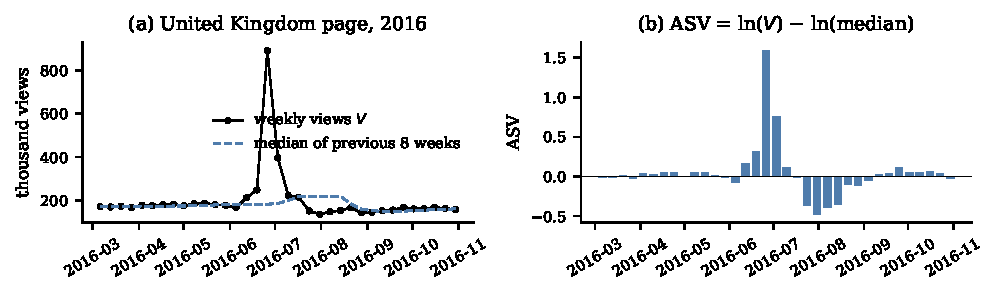
\includegraphics[width=\textwidth]{figures/fig_signal_example.pdf}
\caption{The signal around the Brexit referendum (23 June 2016): weekly views, the eight-week
median baseline, and the resulting ASV.}
\label{fig:signal}
\end{figure}

\section{Additional results}\label{app:tables}
\begin{table}[h]
\centering\small
\caption{Robustness: all pre-specified variations (gross of costs). Placebo (R7): two-sided
$p=\PlaceboP$.}
\label{tab:robustness}
\begin{tabular}{lrrrrr}
\toprule
Test & Weeks & Mean/wk \% & Ann. \% & NW $t$ & Sharpe \\
\midrule
Main specification & 577 & $-$0.073 & $-$3.8 & $-$1.51 & $-$0.45 \\
R1 window 4 weeks & 577 & $-$0.090 & $-$4.7 & $-$2.01 & $-$0.56 \\
R1 window 12 weeks & 573 & $-$0.034 & $-$1.7 & $-$0.71 & $-$0.21 \\
R2 quintiles & 577 & $-$0.099 & $-$5.1 & $-$1.65 & $-$0.49 \\
R2 rank-weighted & 577 & $-$0.067 & $-$3.5 & $-$1.49 & $-$0.44 \\
R3 Economy of pages & 577 & 0.050 & 2.6 & 1.07 & 0.32 \\
R4 2015-09 to 2019-12 & 226 & $-$0.071 & $-$3.7 & $-$0.93 & $-$0.48 \\
R4 2020-01 to 2021-12 & 104 & 0.062 & 3.2 & 0.59 & 0.39 \\
R4 2022-01 to 2026-09 & 247 & $-$0.131 & $-$6.8 & $-$1.73 & $-$0.75 \\
R6 trade one day later & 577 & $-$0.043 & $-$2.2 & $-$0.91 & $-$0.26 \\
R8 high global fear weeks & 288 & $-$0.094 & $-$4.9 & $-$1.29 & $-$0.55 \\
R8 low global fear weeks & 289 & $-$0.052 & $-$2.7 & $-$0.77 & $-$0.34 \\
R9 no English-majority countries & 577 & $-$0.058 & $-$3.0 & $-$1.08 & $-$0.34 \\
\bottomrule
\end{tabular}
\end{table}

\begin{table}[h]
\centering\small
\caption{Leave one country out (R5): High-minus-Low after dropping each ETF.}
\begin{tabular}{lrr@{\hspace{2em}}lrr}
\toprule
Dropped ETF & Ann. \% & NW $t$ & Dropped ETF & Ann. \% & NW $t$ \\
\midrule
EWU (United Kingdom) & $-$4.7 & $-$1.90 & EWZ (Brazil) & $-$3.6 & $-$1.45 \\
MCHI (China) & $-$4.4 & $-$1.74 & ECH (Chile) & $-$3.6 & $-$1.45 \\
EWQ (France) & $-$4.2 & $-$1.72 & EIDO (Indonesia) & $-$3.4 & $-$1.43 \\
INDA (India) & $-$4.2 & $-$1.72 & EWA (Australia) & $-$3.5 & $-$1.39 \\
EWI (Italy) & $-$3.9 & $-$1.60 & EWS (Singapore) & $-$3.4 & $-$1.38 \\
EWP (Spain) & $-$3.8 & $-$1.56 & EPHE (Philippines) & $-$3.5 & $-$1.37 \\
EWJ (Japan) & $-$3.9 & $-$1.54 & EWD (Sweden) & $-$3.3 & $-$1.30 \\
THD (Thailand) & $-$3.8 & $-$1.53 & EWL (Switzerland) & $-$3.3 & $-$1.28 \\
EZA (South Africa) & $-$3.7 & $-$1.53 & EWW (Mexico) & $-$3.2 & $-$1.27 \\
EWM (Malaysia) & $-$3.7 & $-$1.49 & EWG (Germany) & $-$3.2 & $-$1.26 \\
EWC (Canada) & $-$3.8 & $-$1.48 & EWH (Hong Kong) & $-$3.0 & $-$1.18 \\
EWT (Taiwan) & $-$3.7 & $-$1.47 & TUR (Turkey) & $-$2.8 & $-$1.17 \\
EWY (South Korea) & $-$3.5 & $-$1.47 &  & & \\
\bottomrule
\end{tabular}
\end{table}

\begin{table}[h]
\centering\small
\caption{Decision rule (frozen specification, section 11).}
\label{tab:decision}
\begin{tabular}{p{0.55\textwidth}lc}
\toprule
Condition (frozen spec, section 11) & Value & Result \\
\midrule
a) net-of-cost NW $|t|$ $>$ 2 (applied as $t$ $>$ 2, see App. C) & t = $-$6.88 & fail \\
b) same sign as the full sample in $\geq$ 2 of 3 sub-periods (see App. C) & 2 of 3 & pass \\
c) alpha against market, momentum, reversal and dollar factors significant & t = $-$1.56 & fail \\
d) break-even cost $>$ 2 x assumed cost & n/a (gross mean negative) & fail \\
\bottomrule
\end{tabular}
\end{table}

\begin{figure}[h]
\centering
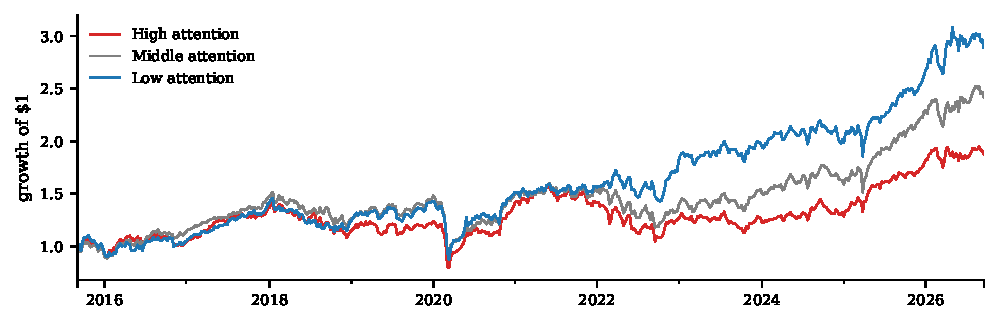
\includegraphics[width=\textwidth]{figures/fig_terciles.pdf}
\caption{Cumulative gross returns of the three tercile portfolios.}
\end{figure}

\begin{figure}[h]
\centering
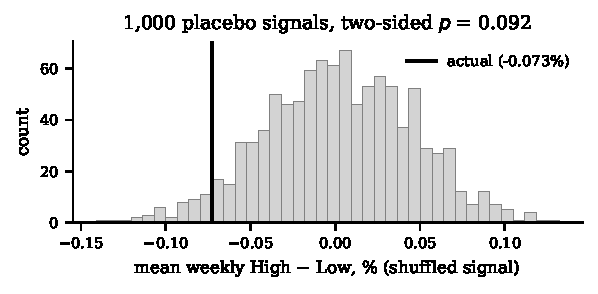
\includegraphics[width=0.6\textwidth]{figures/fig_placebo.pdf}
\caption{Placebo test (R7): mean High-minus-Low return for 1{,}000 signals shuffled across
countries within each week.}
\end{figure}

\textit{Factor premia in the universe (mean weekly return, Newey--West $t$):} market \PremMKT\%
($t=\PremMKTt$), momentum \PremMOM\% ($t=\PremMOMt$), short-term reversal \PremREV\%
($t=\PremREVt$), US dollar \PremUSD\% ($t=\PremUSDt$).

\FloatBarrier
\section{Reproducibility}
Python 3.12 with \texttt{uv}. From the repository root:
\begin{verbatim}
uv sync
uv run python -m cae.universe      # prices + universe filter
uv run python -m cae.views         # Wikipedia views
uv run python -m cae.riskfree      # Ken French risk-free rate
uv run python -m cae.panel         # weekly panel
uv run python -m cae.main_test     # sections 6-7
uv run python -m cae.new_info      # section 8
uv run python -m cae.robustness    # sections 9-11
uv run python -m cae.report_assets # figures and tables for this PDF
uv run python -m cae.check_week EWZ 2022-10-30   # hand-check any row
\end{verbatim}

\section{Use of AI}
\todo{Review and rewrite in your own words.} I used an AI assistant (Claude) to brainstorm signals,
check data availability, write and debug the Python pipeline, and draft the technical sections.
I chose the signal and the design decisions, froze the specification before seeing any result,
inspected every dataset, verified panel rows by hand against the raw data, and kept the
specification unchanged after the results came in. I am responsible for the methods and results.

\end{document}
